\documentclass[12pt]{beamer}
\usetheme{bjeldbak}
\usepackage[utf8x]{inputenc}
\usepackage{ucs}
\usepackage{amsmath}
\usepackage{amsfonts}
\usepackage{amssymb}
\usepackage{graphicx}
\author{Viviana Petrescu}
\title{Machine Learning techniques for predicting molecular properties}

\begin{document}

\begin{frame}
\titlepage
\end{frame}

\begin{frame}
\tableofcontents
\end{frame}

\section{Introduction}
\begin{frame}
\begin{itemize}
\item Compute/predict properties of molecules for materials design\\
Examples: drug discovery, water purification, energy transmission and storage
\item Quantum Chemistry calculations are expensive
\item  Machine Learning could predict properties of molecules at a fraction of the cost
\end{itemize}
\end{frame}

  \begin{figure}[t]
    \centering
    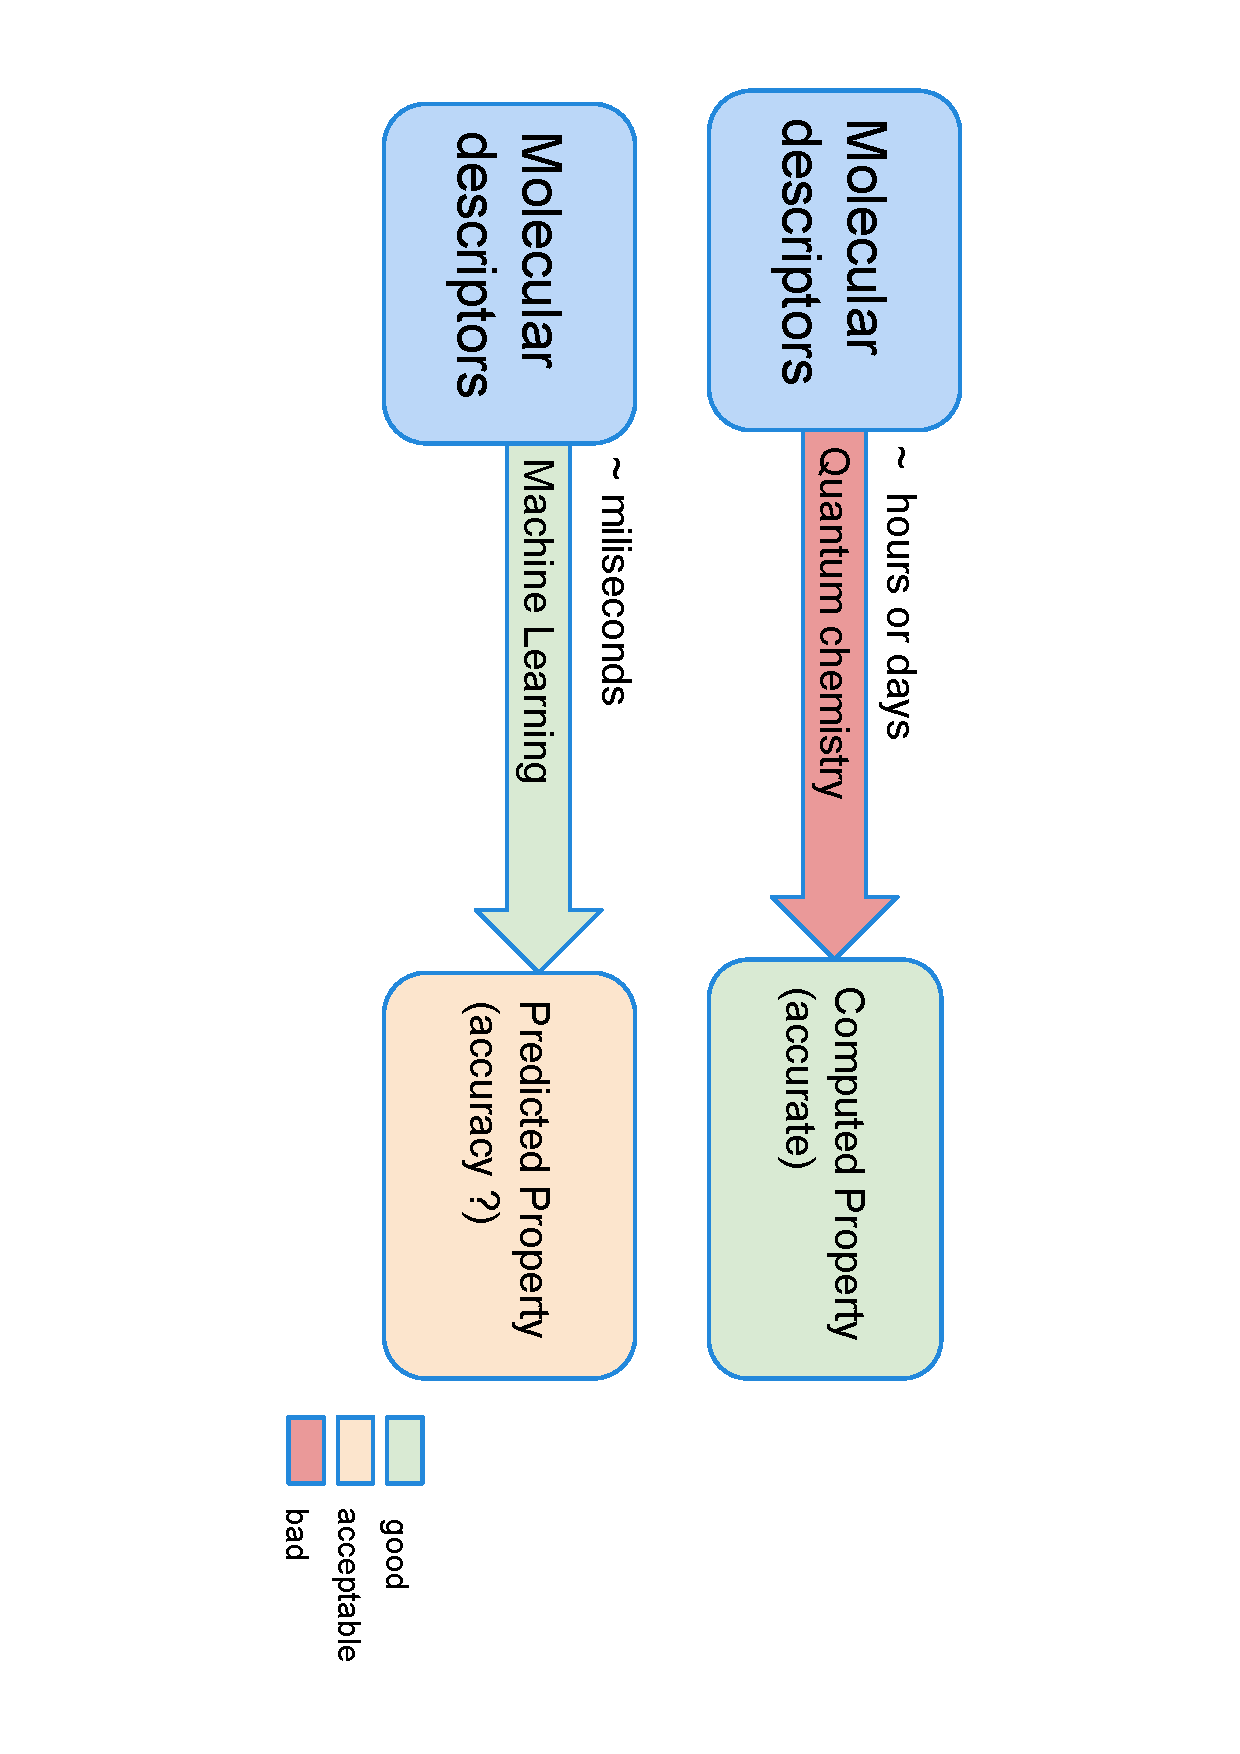
\includegraphics[angle=90,origin=c,height=\dimexpr11\textheight/7\relax]{introslide}
  \end{figure}
  
\section{Background work}
\subsection{Learning Invariant Representations of Molecules for Atomization Energy Prediction}
\begin{frame}
   \frametitle{Molecular descriptors}
\begin{itemize}
\item Desired properties of Molecular Descriptor
\begin{itemize}
\item invariance to atom indexing
\item invariance to rotation and translation
\end{itemize}
\item Coloumb Matrix $[Rupp 2012]$ scales $O(N^2)$

\end{itemize}
\begin{equation}
C(i,j) = \left\{
  \begin{array}{lr}
    0.5*Z_i^{2.4} & i== j\\
    Z_i * Z_j / ||R_i - R_j|| & i\neq j
  \end{array}
\right.
\end{equation}
 $Z_i$ is charge of atom i \\$R_i $ is 3D position of atom $i$

\end{frame}

\begin{frame}
\frametitle{Coloumb Matrix}
Coloumb Matrix descriptor
\begin{itemize}
\item invariant to rotation and translation 
(use     $||R_i - R_j||$                 ) 
\item invariance to atom indexing
	\begin{itemize}
\item Sorted Coloumb Matrix - indexes given by sorting the row norms
\item Random Coloumb Matrix - generate multiple  Sorted Coloumb Matrices  perturbed by noise)
\end{itemize}
\end{itemize}
\end{frame}

\begin{frame}
\frametitle{Random Coloumb Matrix}
Coloumb Matrix descriptor
\begin{itemize}
\item Atomization energy prediction for a dataset of ~7k samples (5.5k training 1.5k testing) with {H,O,C,N,S}
 Multilayer Feed Forward NN with Random Coloumb 
~3.1 kcal/mol MAE  - chemical accuracy level ~1kcal/mol
\end{itemize}
\end{frame}

\subsection{Self-taught Learning: Transfer Learning from Unlabeled Data}
\begin{frame}
  {Introduction}

  Things in a Bulleted List\pause

  \begin{itemize}
  \item Bullets that\pause
  \item Come up\pause
  \item One by one
  \end{itemize}
\end{frame}
\subsection{Information - Theoretic Regret Bounds for Gaussian Process Optimization in the Bandit Setting}
\begin{frame}
  {Introduction}

  Things in a Bulleted List\pause

  \begin{itemize}
  \item Bullets that\pause
  \item Come up\pause
  \item One by one
  \end{itemize}
\end{frame}

\section{Conclusions}

\end{document}